\section[%
Расчет календарно-плановых нормативов и построение стандарт-плана]{
РАСЧЕТ КАЛЕНДАРНО-ПЛАНОВЫХ \\
НОРМАТИВОВ И ПОСТРОЕНИЕ \\
СТАНДАРТ-ПЛАНА
}
\label{sec:kpn}

Основной состав календарно-плановых нормативов ОНПЛ:
\begin{itemize}
  \item такт или ритм потока ( $r_{\text{н.п.}} = 0{,}72$~мин/шт.);
  \item количество рабочих мест по операциям и по всей поточной линии;
  \item скорость движения конвейера и его период;
  \item величина заделов;
  \item длительность производственного цикла, темп поточной линии;
  \item стандарт-план ОНПЛ;
  \item мощность, потребляемая конвейером.
\end{itemize}

\subsection{Определение количества рабочих мест по операциям и по всей поточной линии}
\label{subsec:number_of_employees_calculation}

В таблице~\ref{tbl:technology_synchronization} приведена синхронизация технологического
процесса.

\begin{table} [h!]
  \caption{%
    Синхронизация технологического процесса
  }\label{tbl:technology_synchronization}
  {\small
    \begin{tabular}{| c | c | c | c | m{0.8cm} | m{3cm} | m{3cm} | c |}
      \hline
      \rotatebox[origin=c]{90}{\hspace{2mm}\parbox{3.5cm}{№ операции}} &
      \rotatebox[origin=c]{90}{\hspace{2mm}\parbox{3.5cm}{\vspace{1.5mm}Норма штучного \newline времени, $t_{\text{шт.}}$, мин}} &
      \rotatebox[origin=c]{90}{\hspace{2mm}\parbox{3.5cm}{Коэффициент выполнения \newline норм, $K_{\text{в}}$ }} &
      \rotatebox[origin=c]{90}{\hspace{2mm}\parbox{3.5cm}{\vspace{2mm}Норма штучного \newline времени с учётом \newline $K_{\text{в}}$, $t_{\text{шт.}}^{'}$, мин}} &
      \rotatebox[origin=c]{90}{\hspace{2mm}\parbox{3.5cm}{Такт линии, \newline $r_{\text{п.л.}}$, мин/шт. }} &
      \rotatebox[origin=c]{90}{\hspace{2mm}\parbox{3.5cm}{\vspace{13mm}Расчётное $C_p$ }} &
      \rotatebox[origin=c]{90}{\hspace{2mm}\parbox{3.5cm}{\vspace{13mm}Принятое $C_{\text{пр}}$ }} &
      \rotatebox[origin=c]{90}{\hspace{2mm}\parbox{3.5cm}{Коэффициент загрузки \newline рабочих мест, \newline оборудования, $K_{\text{з}}$ }} \\
      \hline

      1 & 1,42 & 1,00 & 1,42 & 0,72 & \centering 1,96 & \centering 2 & 0,98 \\ \hline
      2 & 0,70 & 1,00 & 0,70 & 0,72 & \centering 0,97 & \centering 1 & 0,97 \\ \hline
      3 & 0,68 & 1,00 & 0,68 & 0,72 & \centering 0,94 & \centering 1 & 0,94 \\ \hline
      4 & 0,70 & 1,00 & 0,70 & 0,72 & \centering 0,97 & \centering 1 & 0,97 \\ \hline
      5 & 2,11 & 1,00 & 2,11 & 0,72 & \centering 2,92 & \centering 3 & 0,97 \\ \hline
      6 & 0,72 & 1,00 & 0,72 & 0,72 & \centering 1,00 & \centering 1 & 1,00 \\ \hline
      7 & 0,67 & 1,00 & 0,67 & 0,72 & \centering 0,93 & \centering 1 & 0,93 \\ \hline
      8 & 2,10 & 1,00 & 2,10 & 0,72 & \centering 2,90 & \centering 3 & 0,97 \\ \hline
      9 & 0,70 & 1,00 & 0,70 & 0,72 & \centering 0,97 & \centering 1 & 0,97 \\ \hline
      \multicolumn{5}{| l |}{\textbf{Итого}} & \centering \textbf{13,54} & \centering \textbf{14} & \textbf{--} \\ \hline

    \end{tabular}
  }
\end{table}

\subsection{Определение периода конвейера и системы адресования}

Период конвейера определяется как наименьшее общее кратное количества рабочих
мест на операциях.
\begin{align*}
  \text{П} = \text{НОК (2, 1, 1, 1, 3, 1, 1, 3, 1)} = 6.
\end{align*}


На рисунке~\ref{pic:conveyor_marker} изображена разметку конвейера.
\begin{figure}[h!]
  \centering
  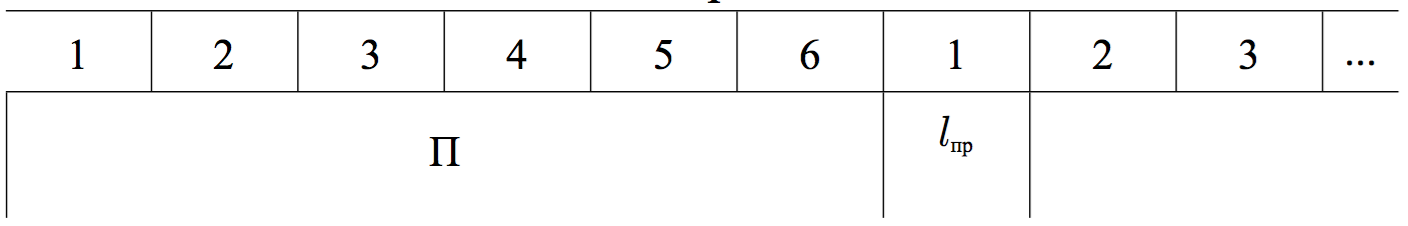
\includegraphics[width=0.8\linewidth]{pic/conveyor_marker}
  \caption{Разметка конвейера}
  \label{pic:conveyor_marker}
\end{figure}

Далее произведём закрепление номеров периода за каждым рабочим местом. Результат
данной операции приведен в таблице~\ref{tbl:numbers_fixation}.

\begin{table} [h!]
  \caption{
    Порядок закрепления номеров за рабочими местами
  }\label{tbl:numbers_fixation}
  {\small
    \begin{tabular}{| c | c | c | c | m{4.9cm} |}

      \hline
        \parbox{2.0cm}{
          \smallskip
          \centering № операции
          \smallskip
        }
      & \parbox{2.0cm}{
          \smallskip
          \centering Число рабочих мест
          \smallskip
        }
      & \parbox{2.0cm}{
          \smallskip
          \centering Номер рабочего места
          \smallskip
        }
      & \parbox{3.5cm}{
          \smallskip
          \centering Число закреплённых номеров за рабочим местом
          \smallskip
        }
      & \parbox{4.9cm}{
          \smallskip
          \centering Последовательность закреплённых номеров за рабочим местом
          \smallskip
        }
      \\ \hline

      \multirow{2}{*}{1} & \multirow{2}{*}{2} & 1 & 3 & 1, 3, 5 \\
                                            \cline{3-5}
                                            & & 2 & 3 & 2, 4, 6 \\
      \hline

      2 & 1 & 3 & 6 & 1, 2, 3, 4, 5, 6 \\ \hline
      3 & 1 & 4 & 6 & 1, 2, 3, 4, 5, 6 \\ \hline
      4 & 1 & 5 & 6 & 1, 2, 3, 4, 5, 6 \\ \hline

      \multirow{3}{*}{5} & \multirow{3}{*}{3} & 6 & 2 & 1, 4 \\
                                            \cline{3-5}
                                            & & 7 & 2 & 2, 5 \\
                                            \cline{3-5}
                                            & & 8 & 2 & 3, 6 \\
      \hline

      6 & 1 & 9  & 6 & 1, 2, 3, 4, 5, 6 \\ \hline
      7 & 1 & 10 & 6 & 1, 2, 3, 4, 5, 6 \\ \hline

      \multirow{3}{*}{8} & \multirow{3}{*}{3} & 11 & 2 & 1, 4 \\
                                            \cline{3-5}
                                            & & 12 & 2 & 2, 5 \\
                                            \cline{3-5}
                                            & & 13 & 2 & 3, 6 \\
      \hline

      9 & 1 & 14 & 6 & 1, 2, 3, 4, 5, 6 \\ \hline

    \end{tabular}
  }
\end{table}


\subsection{Определение длины ленты конвейера}

Если шаг конвейера $l_{\text{пр}}$ на всех операциях принять равным $1{,}1$ м, то
рабочая длина конвейера вычисляется следующим образом:
\begin{align*}
  L_{p} = C_{\text{пр}} \cdot l_{\text{пр}} = 14 \cdot 1{,}1 = 15{,}4~(\text{м}).
\end{align*}

Полная длина ленты конвейера $L_n$ должна быть несколько больше
двойной рабочей длины конвейера и должна быть согласована с условием
распределения, определяемым по формуле:
\begin{align*}
  L_n &= 2 \cdot L_p + \pi \cdot \text{Д} \hspace{5mm} \le \hspace{5mm} K \cdot \text{П} \cdot l_{\text{пр}}, \\
  K   &= \dfrac{L_n}{\text{П} \cdot l_{\text{пр}} }
\end{align*}

При диаметре натяжного и приводного барабанов $ \text{Д} = 0{,}4$ (м) получаем:
\begin{align}
\label{eq:temp}
  L_n &= 2 \cdot 15{,}4 + \pi \cdot 0{,}4 = 32{,}06~(\text{м}) \hspace{5mm} \le \hspace{5mm} 5 \cdot 6 \cdot 1{,}1 = 33~(\text{м}), \\
  K   &= \dfrac{ 32{,}06 }{ 6 \cdot 1{,}1 } = 4{,}86 \approx 5. \nonumber
\end{align}

Видно, что условие~(\ref{eq:temp}) выполняется, значит, шаг конвейера $l_{\text{пр}}$
не нуждается в корректировке.


\subsection{Определение скорости движения ленты конвейера}

Скорость движения ленты конвейера определяется по формуле:
\begin{align*}
  v = \dfrac{ l_{\text{пр}} }{ r_{\text{н.п.}} } = \dfrac{1{,}1}{0{,}72} = 1{,}52~ (\text{м/мин}).
\end{align*}


\subsection{Определение мощности, потребляемой конвейером}

Определим производительность $\rho$ поточной линии по формуле:
\begin{align*}
  \rho = \dfrac{1}{r_{\text{н.п.}}} \cdot 60 = \dfrac{1}{0{,}72} \cdot 60 = 82{,}9~(\text{шт./ч}).
\end{align*}

Часовая производительность конвейера в единицах массы при средней массе
единицы продукции $Q = 0{,}18 $~(кг):
\begin{align*}
  q_r = \rho \cdot Q = 82{,}9 \cdot 0{,}18 = 14{,}93~(\text{кг/ч}).
\end{align*}

Мощность, потребляемая конвейером определяется по формуле:
\begin{align*}
  W &= 1{,}2 \cdot \Big[ \dfrac{ 0{,}16 \cdot L_n \cdot v \cdot Q_k }{ 36 } + \dfrac{ 0{,}16 \cdot L_n \cdot q_r }{ 270 } \Big] , \\
  W &= 1{,}2 \cdot \Big[ \dfrac{ 0{,}16 \cdot 32{,}06 \cdot 1{,}52 \cdot 6 }{ 36 } + \dfrac{ 0{,}16 \cdot 32{,}06 \cdot 14{,}93 }{ 270 } \Big] = 1{,}90~(\text{л.с.}), \\
  P_{\text{уст.}} &= 0{,}736 \cdot W = 0{,}736 \cdot 1{,}90 = 1{,}4~(\text{кВт}).
\end{align*}


\subsection{Расчёт заделов}

На производстве с однопредметной непрерывно-поточной линией создаются заделы
трёх видов: технологический, транспортный и страховой (резервный).

Технологический задел --- количество изделий, которое в каждый момент времени
находится в процессе обработки на рабочих местах. При поштучной передаче изделий
он соответствует числу рабочих мест, таким образом:
\begin{align*}
  Z_{\text{техн}} = C_{\text{пр}} = 14~(\text{шт.}).
\end{align*}

Транспортный задел --- количество изделий, которое в каждый момент времени
находится на конвейере в процессе транспортировки. Для поштучной передаче
изделий определяется по формуле:
\begin{align*}
  Z_{\text{тр}} = C_{\text{пр}} - 1 = 14 - 1 = 13~(\text{шт.}).
\end{align*}

Резервный задел создаётся на линиях с наиболее ответственных или же нестабильных
по времени выполнения операциях, а также на контрольных пунктах. Определяется
по формуле:
\begin{align*}
  Z_{\text{рез}} = \dfrac{t_{\text{рез}}}{r_{\text{н.п.}}}.
\end{align*}

В расчётах $ t_{\text{рез}} $ принимают как $4$ -- $5\%$ штук изделий от сменного
задания. В итоге имеем:
\begin{align*}
  N_{\text{см}} &= \dfrac{30597}{23 \cdot 2} = 665~(\text{шт.}), \\
  Z_{\text{рез}} &= \dfrac{t_{\text{рез}}}{r_{\text{н.п.}}} = \dfrac{665 \cdot 0{,}05}{0{,}72} = 46~(\text{шт.}).
\end{align*}

Общая величина задела определяется как сумма технологического, транспортного и
резервного заделов:
\begin{align*}
  Z_{\text{общ}} = Z_{\text{техн}} + Z_{\text{тр}} + Z_{\text{рез}} = 14 + 13 + 46 = 73~(\text{шт.}).
\end{align*}


\subsection{Расчёт величины незавершенного производства}

Величина незавершенного производства без учёта затрат времени в предыдущем цехе
определяется по формуле:
\begin{align*}
  H_{\text{в}} = Z_{\text{общ}} \cdot \dfrac{\sum\limits_{i=1}^m t_i}{2} = 73 \cdot \dfrac{9{,}8}{2 \cdot 60} = 5{,}96~(\text{нормо-ч}).
\end{align*}

Величина незавершенного производства в денежном выражении определяется по формуле:
\begin{align*}
  H_{\text{з}} = Z_{\text{общ}} \cdot C_z = Z_{\text{общ}} \cdot 0{,}85 \cdot C_{\text{ц}} =
  73 \cdot 0{,}85 \cdot 14{,}94 = 926{,}89~(\text{у.е.}).
\end{align*}

\subsection{Расчёт длительности производственного цикла и построение стандарт-плана}

Длительность производственного цикла определяется графическим (на основе
стандарт-плана) и аналитическим способом. Стандарт-план участка
расположен в приложении~А.

Так как в рассматриваемом примере обработка изделия начинается непосредственно
с первого рабочего места без лишнего интервала движения после последней операции,
то длительность цикла определяется по формуле:
\begin{equation*}
  t_\text{ц} = (2 \cdot \text{С}_{\text{л}} - 1) \cdot r_{\text{н.п.}} = (2 \cdot 14 - 1) \cdot 0{,}72 = 19{,}54~(\text{мин}).
\end{equation*}

